\documentclass[11pt,letterpaper,english]{article}
\usepackage[T1]{fontenc} % Standard package for selecting font encodings
\usepackage{txfonts} % makes spacing between characters space correctly
\usepackage{xcolor} % Driver-independent color extensions for LaTeX and pdfLaTeX.
\usepackage{hyperref}  %The ability to create hyperlinks within the document
%\usepackage{blindtext} % To create text
%\usepackage{mdwlist} % mdwlist for compact enumeration/list items
%\usepackage[pagestyles]{titlesec} % related with sections—namely titles, headers and contents
\usepackage{fancyhdr} % header footer placement

\usepackage[top=1in, bottom=1in, left=1in, right=1in] {geometry} % Margins
\usepackage{graphicx}   % Essential for adding images to you document.

\usepackage{enumitem}  % Helps with the reduce itemize/enumerate separations

\usepackage{sectsty}
\sectionfont{\normalsize}
\subsectionfont{\normalsize}
\subsubsectionfont{\normalsize \it}

\usepackage[font=bf]{caption}
\captionsetup{labelsep=period}

\setlength{\parskip}{\baselineskip}%
\setlength{\parindent}{0pt}%


\pagestyle{fancy} % allows you to use the header and footer commands


\raggedright
\begin{document}

\setlength{\parindent}{0in} % Amount of indentation at the first line of a paragraph.

\pagestyle{fancy} \lhead{Working Title: The Detailed Physical Structure of the Circumgalactic Medium} \rhead{Lead PI: Evan Schneider} \renewcommand{%
\headrulewidth}{0.0pt}

\begin{center}
{\bf PROJECT NARRATIVE (The narrative should not exceed 15 pages)} 
\end{center}

\vspace{-.15in}

%\colorbox{yellow} {\bf {\emph{[Refer to the guidelines for additional instructions for preparing the proposal.]}}}

%\vspace{.15in}

%Visual materials, such as charts, graphs, pictures, etc., are included in the 15-page limit. References {\bf do not} count in the 15-page limit and should be listed after the Project Narrative. URLs that provide information related to the proposal should not be included. {\bf The 15-page limit will be strictly enforced.}  The Project Narrative should address the following points:

\vspace{-.25in}
\section{SIGNIFICANCE OF RESEARCH}
\vspace{-.2in}
%List any previous INCITE award(s) received and discuss the relationship to the work proposed. Explain what advances you expect to be enabled by an INCITE award that justifies an allocation of petascale resources (e.g., anticipated impact on community paradigms, valuable insights into or solving a long-standing challenge, etc.). Place the proposed research in the context of competing work in your discipline or business. The information should be sufficient for peer review in your area of research and also appropriate for general scientific review comparing your proposal with proposals in other disciplines. Potential scientific or business impact is the predominant determinant for awards. This factor will be assessed by a peer-review panel. Also list any previous INCITE award(s) received and discuss the relationship to the work proposed. {\bf This section is typically about 4 pages.}

%When you cite a reference, please insert a number in brackets, as shown here [1], to correspond to its number on the reference list at the end of this template. Please call out the references in numerical order and list them in the same way. The reference list will {\bf not} count toward the 15-page limit.
%(Placeholder text. This section should be about {\bf 1 page}.)

Large-scale simulations of galaxy formation in the universe have made enormous strides in the past decade, with models that are now able to reproduce a remarkably wide range of observations.  However, the ability of these models to make predictions is hampered by their difficulty in modeling the small-scale gas physics that regulate how baryons get in to -- and out of -- galaxies, as well as how much of it cools to forms stars.   Currently the codes used for these simulations use sub-grid recipes that must be calibrated against observations, strongly reducing their ability to constrain fundamental physics such as the nature of dark energy or dark matter.  Some of the most challenging sub-grid physical models involve the multi-phase gas in and around galaxies.   In the past, such models could not be developed or tested through direct simulation due to the large range of scales present in astrophysical, multi-phase flows; however, recent advances in hardware and software have now made it possible to carry out the numerical models required to understand these flows. {\bf This proposal lays out a systematic plan that harnesses the leadership computing facility Titan XK7 and our GPU-native hydrodynamical simulation code Cholla [REF] in order to understand the development and evolution of multi-phase, turbulent astrophysical gas flows by resolving the relevant scales for the first time. }

Many astrophysical systems produce turbulent, pressure-confined diffuse gas which is prone to the formation of thermal instabilities.  Such systems include the circumgalactic medium of galaxies, the intracluster medium of X-ray clusters, and even the interstellar medium, and so play a key role in the evolution of many systems.  While the linear evolution of the thermal instability in extremely simplified systems has been well-studied, we still lack a good understanding of how this gas evolves in the non-linear stages and how the multi-phase state saturates.  A wide range of scales is likely to be involved and yet the cold clouds that form will be widely distributed, a combination which requires high resolution throughout the domain.  We are particularly motivated by the circumgalactic medium (CGM), the diffuse gas which lies outside of the disk of the galaxy and yet is still gravitationally bound to the overall system (which is dominated in mass by dark matter).  While this gas emits radiation very faintly and is difficult to detect directly, recent observations of background sources have been used to probe the CGM by measuring absorption lines of hydrogen and other elements.  Such work has produced a conundrum, with the detection of gas that it is at a wide range of temperatures and ionization states, something that cosmological simulations generally cannot reproduce, perhaps because they lack the resolution to model multiphase gas.

Here, we propose to carry out a set of simulations of a small region of the CGM (we focus on the CGM in this proposal, but we expect our results to be much more widely applicable).  As described in more detail below, we have identified both the smallest and the largest scales that we believe we need to simulate in order to develop a physical understanding of the dynamics of cooling, turbulent gas.  The requirements are severe, with a ratio of largest to smallest length scales of order $10^{3-4}$; moreover, because of the turbulent nature of the gas, the cold clumps which condense out can do so anywhere and at many places nearly simultaneously, with no preferred geometry.  This means that we simply need to resolve the entire region at high resolution, a requirement which has prevented this from being done until now.  We will perform simulations to first determine the require resolution to numerically converge on the distribution of gas phases (our key takeaway), and then systematically vary the mean properties of the box (primarily density and velocity dispersion of the turbulent gas) based on galaxy simulations.  From this, we will develop both a physical understanding of the multiphase gas as well as simple model that can included in large-scale simulations.  In this way, we aim to make the cosmological simulations much less dependent on tuned sub-grid models and therefore more predictive.


%This first section should be broad enough for a general audience comparing our proposal with those in other disciplines.

%Broad science overview paragraph, including bold (literally and figuratively) thesis statement.

%Brief statement of the problem.

%Brief description of the proposed simulations (solution).

%Brief description of the impact of the project on the community.

(Brief description of previous awards and their relation to this proposal.)

Three of the foremost questions in modern astrophysics are (i) what fuels the growth of galaxies, (ii) what quenches the growth of some galaxies, and (iii) where does most of the matter in universe reside. The flow of gas through the circumgalactic medium (CGM) -- the dilute gas that surrounds galaxies and fills their dark matter halos -- regulates the galaxy growth over cosmic time. 
%GB: The above paragraph got added while I was working on mine -- maybe a conflict?


\vspace{-.25in}
\subsection{Scientific Motivation}
\vspace{-.2in}

The circumgalactic medium (CGM) plays an outsize role in the modern picture of galaxy formation: gas enters into the CGM from the intergalactic medium, often via (possibly cold) filamentary flows and material stripped from merging halos, it accretes onto the star forming galaxy at the center of the halo, fueling star formation, and it receives ejected gas via stellar and black-hole feedback (see \cite{Tumlinson17} and \cite{Putman12} for recent reviews). % more background coming...

(Placeholder text. This section should be about {\bf 2 pages}.)

This is where we really dig in to the science. The level should be appropriate for peer review in astrophysics.

Outline the science background. I like to start with an interesting observation, followed by a problem, followed by our solution to the problem. Possible structure:
\begin{itemize}
\item{Background: recent observational studies of the CGM (COS and friends)}
\item{Theoretical puzzle: how to explain the cool gas in galaxy halos? Observations point towards small-scale structures, well below the resolution limit of current cosmological simulations.}
\item{Theoretical solution: small volume-filling cool structures seeded by turbulence + thermal instability in the CGM. Possibly very small - $c_\mathrm{s} t_\mathrm{cool}$ of order a few to tens of parsecs (see Figure~\ref{fig:cs_tcool}).}
\item{Logical numerical study: simulations of patches of the CGM with driven turbulence and astrophysical cooling, with $c_\mathrm{s} t_\mathrm{cool}$ resolved. For driving scales of order 1 kpc, this will require very high resolution boxes.}
\item{What will be gained from the study.}
\item{Additional benefits to the community (e.g. better physical understanding of CGM phase structure to inform observations, subgrid model for cosmological simulations, etc..}
\end{itemize}

%\begin{figure}[h]
%\centering
%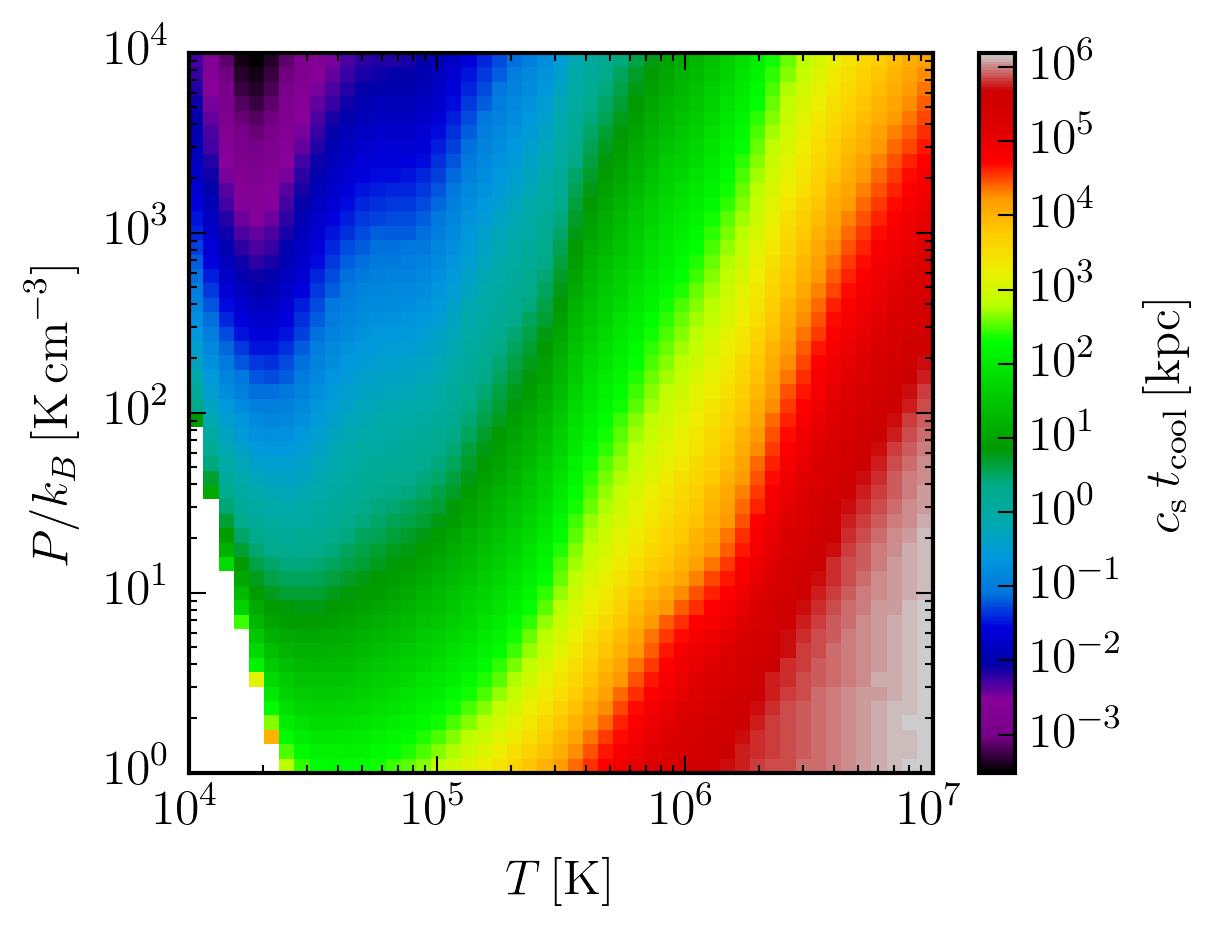
\includegraphics[width=4.52in, height=3.08in, keepaspectratio=true]{cs_tcool_P_T_3.png}
%\caption{This figure justifies our resolution requirements. Would be nice to have the minimum length scale in one panel (as shown), and a figure justifying the box size in another panel (if we can think of an appropriate figure).}
%\label{Fig1}
%\end{figure}


\begin{figure}[h]
    \centering
    \begin{minipage}{0.6\textwidth}
        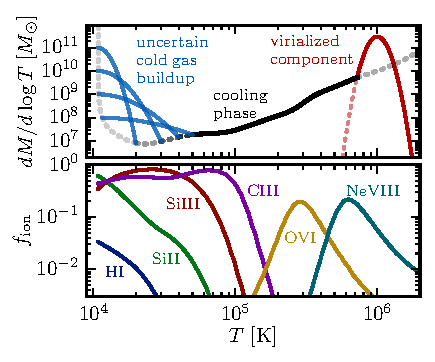
\includegraphics[width=0.975\textwidth]{../figures/dMdlogT_picture_ion_all_P100_broad_narrow_3in.pdf} 
    \end{minipage}\hfill
    \begin{minipage}{0.4\textwidth}
        \centering
\caption{\textit{Top}: Phase distribution showing the contribution from the virialized, cooling, and cold components. The sensitivity of the coldest phase to resolution and microphysics lead to changes in its distribution. \textit{Bottom}: Ion fraction for various ions that are or can be observed in the CGM of low redshift galaxies assuming they are at a pressure of $P/k_B = 100\,\mathrm{K\,cm}^{-3}$. Small changes to the phase structure at low temperatures can have a major impact on the integrated ion column densities and therefore the inferred CGM properties.\label{fig:multiphase}} 
\end{minipage}
\end{figure}


\begin{figure}[h]
    \centering
    \begin{minipage}{0.45\textwidth}
	\caption{ The largest and smallest relevant length scales as a function of pressure. The dark blue line shows $\ell_{\rm cool} = c_{\rm s} \, t_{\rm cool}$, which is the expected minimum cold cloud size \cite{McCourt18} that we would want to resolve by at least several grid cells. The orange dashed line traces $R_{\rm CGM}$, the characteristic radius in the CGM at a given pressure from global CGM simulations \cite{Fielding17}. In order accurately model the multi-phase structure of the CGM it is necessary to include the dynamics on scales roughly $1/2 - 1/10 \ R_{\rm CGM}$. The range of scales necessary to capture, therefore, ranges from roughly a few 10s to a few 1000s. \label{fig:cs_tcool}}
    \end{minipage}\hfill
    \begin{minipage}{0.55\textwidth}
        \hspace{0.3cm} 
        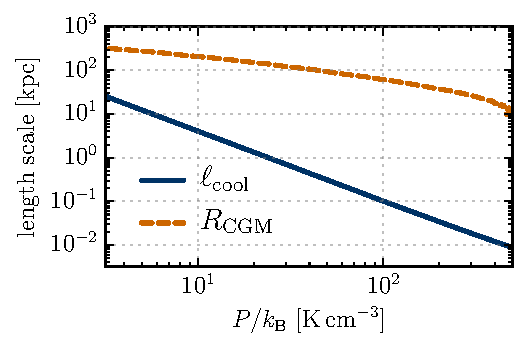
\includegraphics[width=1.1\textwidth]{../figures/length_scales_sim.pdf} 
    \end{minipage}
\end{figure}


\begin{figure}[h]
    \centering
    \begin{minipage}{0.6\textwidth}
        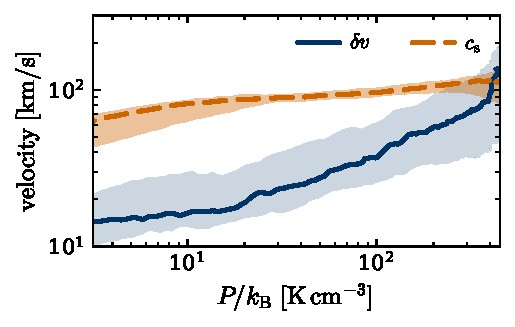
\includegraphics[width=0.975\textwidth]{../figures/velocity_P.pdf} 
    \end{minipage}\hfill
    \begin{minipage}{0.4\textwidth}
        \centering
\caption{Characteristic values of the velocity dispersion (dark blue line; $\delta v = \sqrt{\langle v^2 \rangle - \langle v \rangle^2}$) and the sound speed (orange dashed line; $c_{\rm s}$) relative to the volume average pressure from global CGM simulations \cite{Fielding17}. The shaded regions trace the one sigma temporal variability around the median values over the full 9 Gyr duration of the simulation, thus demonstrating the need to study how the phase structure changes for different choices of the Mach number $\mathcal{M} = \delta v /  c_{\rm s}$. \label{fig:velocities}} 
\end{minipage}
\end{figure}



\vspace{-.25in}
\subsection{Results from Previous INCITE Awards and Relation to Current Proposal}
\vspace{-.2in}

(Placeholder text. This section should be {\bf < 1 page}.)

(Evan will add more here.)

Previous awards include DD projects AST107 "Scaling the GPU-enabled Hydrodynamics Code Cholla to the Power of Titan" and AST119 "Extending the Physics of the GPU-Enabled CHOLLA Code to the Power of Titan" (co-I Schneider) and INCITE project AST125 "Revealing the Physics of Galactic Winds with Petascale GPU Simulations" (co-PI Schneider). Results from project AST107 included the first demonstration of {\tt Cholla} at petascale. AST119 allowed the development of GPU-accelerated radiative cooling and associated research into the cloud-wind problem, through which we demonstrated that the cool gas in the CGM cannot be directly explained by ram pressure acceleration of dense disk material \cite{Schneider17}. The ongoing INCITE project AST125 has produced the most detailed numerical models of multiphase galactic winds ever, but the simulations only extend out to 10 kpc, and thus cannot be used to determine what happens to the gas in the wind once it reaches the CGM. There are strong indications that starburst winds are a driver of the large-scale turbulence to be investigated via this project, see also \cite{Fielding17}).


\vspace{-.25in}
\section{RESEARCH OBJECTIVES AND MILESTONES }  
\vspace{-.2in}
%Describe the proposed research, including its goals and milestones and the theoretical and computational methods it employs. Goals and milestones should articulate simulation and developmental objectives and be sufficiently detailed to assess the progress of the project for each year of any allocation granted. Milestones should correlate with those in the milestone table. It is especially important that you provide clear connections between the project's overarching milestones, the planned computational campaign, and the compute time expected to be required for this campaign (e.g., should correlate with those in the ``Use of Resources Requested''). {\bf This section is typically about 6 pages.}

(Placeholder text. This section should be about {\bf 6 pages}.)

This section needs a lot of filling out. Basically, this is where we describe the set of simulations we plan to do, and why we're doing them. I've come up with a baseline set of simulations that I think we could do based on the computational time, and a baseline set of objectives and milestones. In describing the simulations, we should include density and temperature projections (I've put some that I generated in as placeholders at the moment). I think some of Drummond's density / temperature pdfs would be good in this section as well, to help describe the analysis we will do and how it relates to our research objectives.

\begin{table}[h]
%\centering
\vspace{-.12in}
\begin{tabular}{|l|l|} 
\multicolumn{2}{l}{\bf{Table 1: Research Objectives}}\\
\hline
\textbf{RO.A} & Determine the effects of resolution on current numerical attempts to characterize the CGM. \\ \hline
\textbf{RO.B} & Describe the physical nature (phase structure, cloud size scales, velocity coherence length etc.) \\
& of gas in the circumgalactic medium for a range of physical pressures. \\ \hline
\textbf{RO.C} & Develop a connection between the state of the CGM and other relevant galaxy properties, \\
& both simulated and observable (e.g. halo mass, star-formation rate, etc.). \\
\hline
\end{tabular}
\end{table}

\begin{figure}[h]
    \centering
    \begin{minipage}{0.33\textwidth}
%        \centering\vspace*{-.25cm}
\caption{Two dimensional slice through a preliminary three dimensional local simulation showing the temperature of a small patch of CGM with a representative average density, temperature, and velocity field. This 1 kpc per side simulation demonstrates the rich multiphase structure that develops via turbulence and thermal instability on scales well below what is obtainable with cosmological zoom-in simulations. Accounting for this unresolved structure will bring global CGM simulations \cite{Fielding17} into agreement with observations. \label{fig:CGMpatch}}
    \end{minipage}\hfill
    \begin{minipage}{0.67\textwidth}
        \hspace{0.3cm} 
        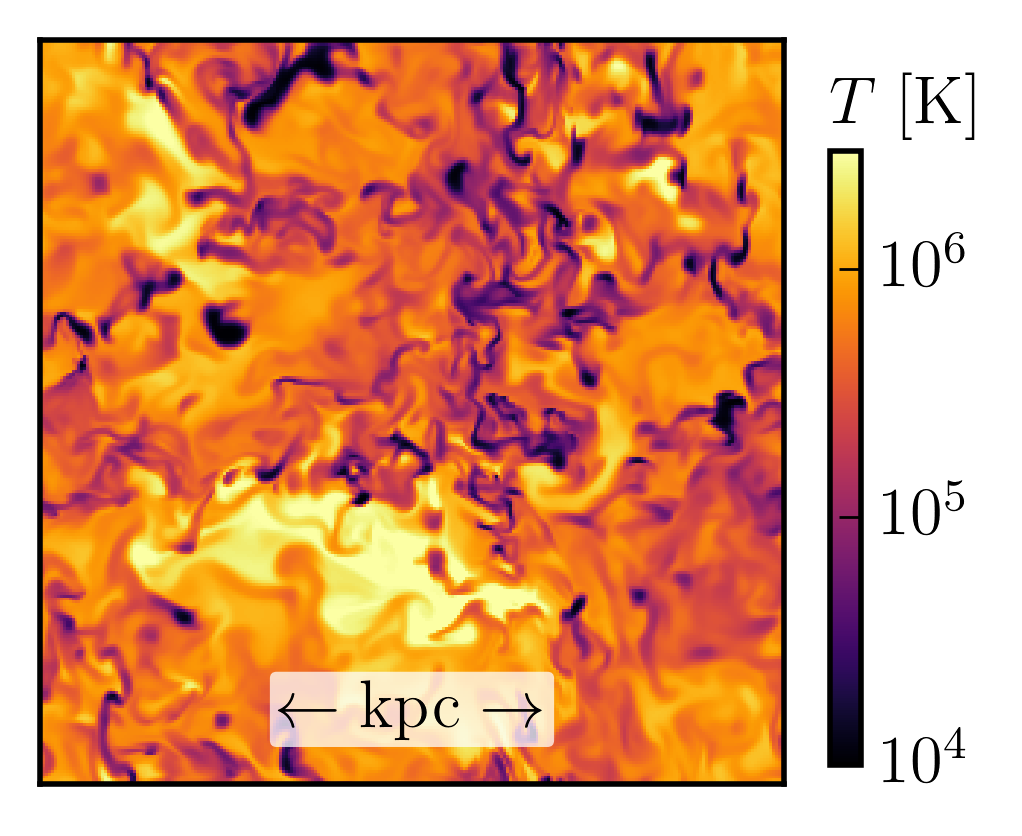
\includegraphics[width=1.04\textwidth]{T_proposal.png} 
    \end{minipage}
\end{figure}

\begin{table}[h]
%\centering
\vspace{-.12in}
\begin{tabular}{|l|p{4.6in}|l|} 
\multicolumn{3}{l}{\bf{Table 2: Research Milestones}}\\
\hline
\multicolumn{2}{|l|}{\bf Milestone} & {\bf Objective} \\ \hline
\multicolumn{3}{|c|}{\it Quarter 1} \\ \hline
\textbf{RM.A} & Develop "fiducial" turbulent CGM model and run resolution study, including first petascale simulation of the CGM. & RO.A , RO.B \\ \hline
\multicolumn{3}{|c|}{\it Quarter 2} \\ \hline
\textbf{RM.B} & Run suite of moderate resolution turbulent box simulations to explore relevant parameter space. & RO.B, RO.C\\ \hline
\multicolumn{3}{|c|}{\it Quarter 3} \\ \hline
\textbf{RM.C} & Run additional extreme resolution models (as informed by parameter study) to produce a state-of-the-art suite of numerical simulations to be used for comparison to observational and theoretical models of the circumgalactic medium. & RO.A, RO.B, RO.C \\ 
\hline
\end{tabular}
\end{table}

\vspace{-.25in}
\subsection{Heading 2 (optional)}
\vspace{-.2in}

Insert paragraph(s).

\vspace{-.25in}
\subsubsection{Heading 3 (optional)}
\vspace{-.2in}

Insert paragraph(s).

\vspace{-.25in}
\section{COMPUTATIONAL READINESS}
\vspace{-.2in}

%Proposals will be assessed on the need for, readiness to use, and reasonableness of the request for resources. Proposals should summarize the requirement(s) that best exemplifies the proposed computational work. Leadership targets in the INCITE program typically include one or both of the following categories:
%\begin{itemize}[noitemsep,topsep=0pt]
%\item Use of 20 percent or more of the system for production calculations. Simulations, data, and/or learning science projects should use a significant fraction of LCF resources, which can include compute, memory, network or disk, for example. Parameter sweeps, ensembles, design of experiments, and other statistical methods that require large numbers of discrete or loosely coupled simulations may be considered capability-class campaigns. See the FAQs for details and qualifiers.\\
%\item Specific architectural needs that can only be met by the LCF.
%\end{itemize}
%\vspace{.1 in}
Placeholder text. This section, including the following subsections, is typically about \textbf{5 pages}.

\vspace{-.25in}
\subsection{Use of Resources Requested}
\vspace{-.2in}

%Describe your proposed production simulations and state how the runs are tied to each of your project's goals and milestones (Section 4, "Milestone Table"). Note that the Milestone Table should be a summary of the detailed information provided here.  For the research campaign you plan to carry out, provide a

%\begin{enumerate}[noitemsep,topsep=0pt]
%\item Description of what computations are going to be run and how they relate to the research/development objectives and milestones given above;
%\item Description of processor/node use for large runs (e.g., 10,000-hour run with 100 nodes, or ten 10-hour runs with 10,000 nodes, for a 1,000,000 node-hour allocation) and for the GPU-accelerated resources, indicate which of these production simulations employ the GPUs. 
%\item Clear, detailed explanation as to how you calculated the requested number of node-hours;
%\item Summary of your anticipated annual burn rate (e.g., linear or with periods of peak usage).  
%\item For projects that are in the space of data, learning or other emerging technologies, a description of how the unique LCF resources (e.g. the unique node or system architecture, inter-node parallelism, intra-node parallelism, the deep memory hierarchy including SSDs, high band-width network, or data storage) enable your campaign.\\
%\end{enumerate}

%\vspace{.1in}
%Also describe the data requirements of your campaign, including:

%\begin{enumerate}[noitemsep,topsep=0pt]
%\setcounter{enumi}{4}
%\item Estimate and breakdown of the anticipated cumulative size of stored data, in scratch and long-term archival storage, at the end of the requested award. 
%\item Description of the effective lifetime of your stored data.  If the lifetime varies, show the breakdown by the total size used.  Explain the reason for the lifetime.
%\item Description of the data, including the expected size of the data, which will be transferred into or out of the center.  Describe what tools for transferring the data from external sources will be used.
%\item Description of the tools for data storage, compression (reduction), and analysis that you currently use. Describe whether the tools and/or applications needed are ready or whether there are new capabilities or features that must be developed.
%\item If you are intending to make any fraction of the data generated public, specify:
%\begin{enumerate}[noitemsep,topsep=0pt]
%\item How much data and the scientific purpose
%\item What tool will be used to share the data
%\item From where will the data be shared\\
%\vspace{.1in}
%If at any point during your project the sum of your data storage needs in the scratch filesystems exceed 500 terabytes, specific justification is required. 

%NOTE: The LCF data management policies can be found at

%OLCF:  {\href{https://www.olcf.ornl.gov/computing-resources/data-management/data-management-user-guide/}{https://www.olcf.ornl.gov/computing-resources/data-management/data-management-user-guide/}}

%ALCF:  {\href{http://www.alcf.anl.gov/user-guides/data-policy}{http://www.alcf.anl.gov/user-guides/data-policy}}
%\end{enumerate}
%\end{enumerate}

Our program for simulating the CGM requires two classes of simulations - petascale simulations where we fully resolve the minimum length scale set by thermal instability, as well as a set of moderate-resolution simulations that will allows us to sample the parameter space of CGM conditions. We note that while we refer to them as moderate resolution, these simulations will still be orders of magnitude better resolution than any previous simulations of the CGM, and therefore will provide highly valuable scientific content. Since all of
our calculations will use the GPU-native code {\tt Cholla}, each of these simulations will require large numbers of GPUs (4096--16,384) as provided by the Titan XK7 system.

(Evan will add more here.)

%Grid size = 2048x2048x2048
%4096 GPUS
%128^3 cells / GPU
%Box size = 1.024kpc^3
%spatial resolution: 1.024kpc / 2048 = 0.5pc
%dt = 1ky?
%each time step ~500ms
%cooling time ~30 Myr
%node hours for 100 Myr = 0.415*1e5*4096 = 56,889 node-hours

%Grid size = 4096x4096x4096
%16,384 GPUS
%128x128x256 cells / GPU
%Box size = 1.024kpc^3
%spatial resolution: 1.024kpc / 4096 = 0.25pc
%dt = 1ky?
%each time step ~1000ms
%cooling time ~30 Myr
%node hours for 100 Myr = 1.0*1e5*16,384 = 455,111 node-hours

\begin{table}[h]
%\centering
\vspace{-.12in}
\begin{tabular}{|l|p{2in}|p{1in}|p{0.7in}|p{0.5in}|p{0.7in}|} 
\multicolumn{6}{l}{\bf{Table 3: Research Simulations}}\\
\hline
\multicolumn{2}{|l|}{\bf Simulation Type and Details} & {\bf Objective / Milestone} & {\bf Resolution} & {\bf Titan Nodes} & {\bf Titan Node Hours} \\ \hline
\multicolumn{6}{|c|}{\it Quarter 1: 0.5M node hours} \\ \hline
\textbf{RS.A} & Fiducial CGM Petascale Simulation and Resolution Study & RO.A, RO.B & $N=1024^3$ & 8 - 16,384 & 0.5M\\ \hline
\multicolumn{6}{|c|}{\it Quarter 2: 0.7M node hours} \\ \hline
\textbf{RS.B - M} & Parameter Study, set of 12 moderate resolution simulations & RO.B, RO.C & $N=2048^3$ & 4096 & 0.7M\\ \hline
\multicolumn{6}{|c|}{\it Quarter 3: 1.5M node hours} \\ \hline
\textbf{RS.N - P} & Three additional petascale simulations based on results of parameter study & RO.A, RO.B, RO.C & $N=4096^3$ & 16,384 & 1.5M\\ \hline
\end{tabular}
\end{table}


\vspace{-.25in}
\subsection{Computational Approach}
\vspace{-.2in}


%Provide a detailed description of your computational approach, including a discussion of the state of the art in the field. The description should also mention:

%\vspace{-.25in}
%\begin{enumerate}
%\item Particular libraries required by the production and analysis software, algorithms and numerical techniques employed (e.g., finite element, iterative solver), programming languages, and other software used.
%\item Parallel programming model(s) used (e.g., MPI, OpenMP/Pthreads and vector intrinsics (QPX/AVX-512) for BG/Q or Xeon Phi; MPI, OpenMP/Pthreads, CUDA, OpenACC or AVX intrinsics for XK7).
%\item Project workflow including the role of analysis and visualization; identify where the analysis will be done and any potential bottlenecks in the analysis process.  Describe any analysis and/or data reduction tools used.
%\item Software workflow solution (e.g., pre- and postprocessing scripts that automate run management and analysis) to facilitate this volume of work.
%\item I/O requirements (e.g., amount, size, bandwidth, etc.) for restart, analysis, and workflow. Highlight any exceptional I/O needs.
%\item For projects that are in the space of data, learning or other emerging technologies, a detailed description of the efficacy of software or proposed software which will be developed to utilize the requested resources and whether that software is already installed and working on the LCF resources
%\end{enumerate}

{\bf Overview}:\\
{\tt Cholla} is a Godunov\cite{Godunov59}-based, finite-volume, Eulerian grid 
hydrodynamics code that takes advantage of the massively parallel computing power of GPUs \cite{Schneider15}. 
In order to harness this power, {\tt Cholla} was designed with the operation of the GPU in mind. 
{\tt Cholla} consists of a set of C/C++ routines that run on the CPU 
(the ``host'') plus functions called kernels that execute on one or
more GPUs (the ``device''). The device kernels and the host functions that call them are written in CUDA C, an extension to the C language introduced by NVIDIA. All of the CUDA functions are contained in a separate hydro module so that they can be compiled independently with the NVIDIA {\tt nvcc} compiler. %In addition, we have written a C/C++ version of the hydro module that performs the same calculations as all of the GPU kernels, so it is possible to run {\tt Cholla} without using graphics cards. We use this mode for testing, but for performance applications the structure of the code is optimized for use with GPUs.

{\tt Cholla} represents the state-of-the-art for astrophysical hydrodynamics
simulations
on a fixed Cartesian mesh. The physical modeling used by {\tt Cholla} 
includes a range of reconstruction methods (including both the characteristics PPM model of {\tt Athena} and the primitive PPM model used
by, e.g., {\tt Flash}), a variety of exact and approximate Riemann solvers,
and two unsplit integrators (Constrained Transport Upwind and Van Leer).
As demonstrated in \cite{Schneider15}, the use of GPUs enables
{\tt Cholla} to achieves a $\sim50\times$ speed-up (1 GPU vs. 1 CPU core)
over CPU-only codes performing hydrodynamics with a similar level of physical fidelity.


Given the typical power of a single GPU, small problems can easily be run on 
a single host/device pair. For large problems like those considered
by
this proposal, {\tt Cholla} can be run using the MPI library to perform message passing between processes that govern separate computational subvolumes. Each subvolume is treated as a self-contained simulation volume for the duration of each simulation time step. Portions of our algorithm that require information from potentially distant cells in the global simulation volume are carried out on the host. The main host functions set initial conditions, apply boundary conditions, and perform any interprocess communications. Parts of the calculation that only require information from nearby cells are carried out on the device. Because the bulk of the computational work resides in the hydrodynamics integration module that requires a stencil containing only local cells, essentially all of the hydrodynamical computations are performed on the GPU.
The steps in the {\tt Cholla} algorithm are listed below.
\vspace{-.1in}
\begin{enumerate}\itemsep0pt
\item Initialize the simulation by setting the values of the conserved fluid quantities for all cells in the simulation volume, and calculate the first time step.
%\vspace{-.1in}

\item Transfer the array containing the conserved variables and other fluid variables of interest (e.g. the gas thermal energy) to the GPU. This array contains all the fluid variables that are being tracked for every cell in the simulation volume.
%\vspace{-.1in}

\item Perform the hydrodynamic integration (using either the CTU or Van Leer method) on the GPU, including updating the conserved variable array and computing the next time step.
%\vspace{-.1in}

\item Transfer the updated fluid variable array back to the CPU.
%\vspace{-.1in}

\item Apply the boundary conditions. When running an MPI simulation, this step may require interprocess communication to exchange information for cells at the edges of subvolumes.
%\vspace{-.1in}

\item Output simulation data if desired.
%\vspace{-.1in}

\end{enumerate}

The initialization of the simulation is carried out on the host(s). The initialization includes setting the values of the fluid variables for both the real and the ghost cells according to the conditions specified in a text input file. Ghost cells are a buffer of cells added to the boundaries of a simulation volume to calculate fluxes for real cells near the edges. The number of ghost cells reflects the size of the local stencil used to perform fluid reconstruction. Because updating the ghost cells at each time step may require information from cells that are not local in memory, the values of the ghost cells are set on the host before transferring data to the GPU.

Once the simulation volume has been initialized on the CPU, the hydrodynamical calculation begins. The host copies the fluid variable array onto the device. Because the GPU has less memory than the CPU, the fluid variable array associated with a single CPU may be too large to fit into the GPU memory at once. If so, {\tt Cholla} uses a series of 
subgrid splitting routines to copy smaller pieces of the simulation onto the GPU and carries out the hydrodynamics calculations on each subvolume. At the end of the hydro calculation the next time step is calculated on the device using a GPU-accelerated parallel reduction. The updated fluid variables and new time step are then transferred back to the host. The host updates the values of the ghost cells using the newly calculated values of the real cells, and Steps 2-5 repeat until the desired final simulation time is reached.

The design of the massively parallel algorithm implemented by {\tt Cholla} allows execution on multiple GPUs simultaneously. {\tt Cholla} can thereby gain a multiplex advantage beyond the significant computation power afforded by a single GPU. This additional parallelization is implemented using the MPI library. The global simulation volume is decomposed into subvolumes, and the subvolumes are each assigned a single MPI process. In {\tt Cholla}, each MPI process runs on a single CPU that has a single associated GPU, such that the number of MPI processes, CPUs, and GPUs are always equal. When the simulation volume is initialized, each process is assigned its simulation subvolume and surrounding ghost cells. Since the hydrodynamical calculation for every cell is localized to a finite stencil, only the ghost cells on the boundary of the volume may require updating from other processes via MPI communication every time step. Compared with a simulation done on a single CPU/ GPU pair, additional overheads for a multi-process simulation can therefore include MPI communications needed to exchange information at boundaries and potential inefficiencies in the GPU computation introduced by the domain decomposition. While domain decomposition influences communications overheads in all MPI-parallelized codes by changing the surface area-to-volume ratio of computational subvolumes, domain decomposition additionally affects the performance of a GPU-accelerated code by changing the ratio of ghost to real cells in memory that must be transferred to the GPU. Since memory transfers from the CPU to the GPU involve considerable overhead, domain decompositions that limit the fraction of ghost cells on a local process are favorable.


\vspace{-.25in}
\subsection{Parallel Performance}
\vspace{-.2in}

%Provide direct evidence, {\bf including supporting quantitative data}, for your production application?s parallel performance for the intended campaign. Ideally, the proposing team will demonstrate proficiency with their application codes, will have generated the performance data on the LCF resource requested or another comparable resource, and these data will be representative of the entire workflow of the project proposed. If you cite work by others, explain why it is applicable here. You should use the application code you intend for the production work, not a related code. Data for sample systems not related to the intended research is undesirable. Performance benchmarking should reflect all I/O and workflow requirements. Parallel performance data in either strong or weak scaling mode must be provided. Explain how the strong or weak scaling applies to the proposed work. 

%NOTE: You may apply for a startup account at one of the centers to conduct performance studies. Applications are available at

%ALCF: {\href{http://www.alcf.anl.gov/getting-started/apply-for-dd}{http://www.alcf.anl.gov/getting-started/apply-for-dd}}

%OLCF: {\href{http://www.olcf.ornl.gov/support/getting-started/olcf-director-discretion-project-application}{http://www.olcf.ornl.gov/support/getting-started/olcf-director-discretion-project-application}}

The ability to run extremely high resolution static grid hydrodynamic simulations was the primary motivation for creation of the {\tt Cholla} code, and as such, weak scaling performance has been a high priority at all stages of development. Our DD Project AST107, ``Scaling the GPU-enabled Hydrodynamics Code {\tt Cholla} to the Power of Titan'', allowed us to test the parallel performance of the code in the petascale regime, with the excellent results shown in the left panel of Figure~\ref{fig:weak_scaling}. These tests followed the adiabatic propagation of an acoustic wave across the grid for a constant number of time steps. The total sizes of the simulations were scaled such that each GPU was assigned $\approx 322^3$ cells. Figure~\ref{fig:weak_scaling} displays the scaling of the total simulation runtime, as well as the breakdown between the hydrodynamics integration, all of which is computed on the GPU, and the necessary communication between MPI processes to exchange boundary cell information. The jaggedness of each scaling reflects the fact that some domain decompositions have more favorable surface-to-volume ratios than others, however we emphasize the the total scaling remains roughly flat out to 16,384 GPUs (simulating $>0.5$T cells), on roughly 90\% of the Titan system.

\begin{figure}[h]
\centering
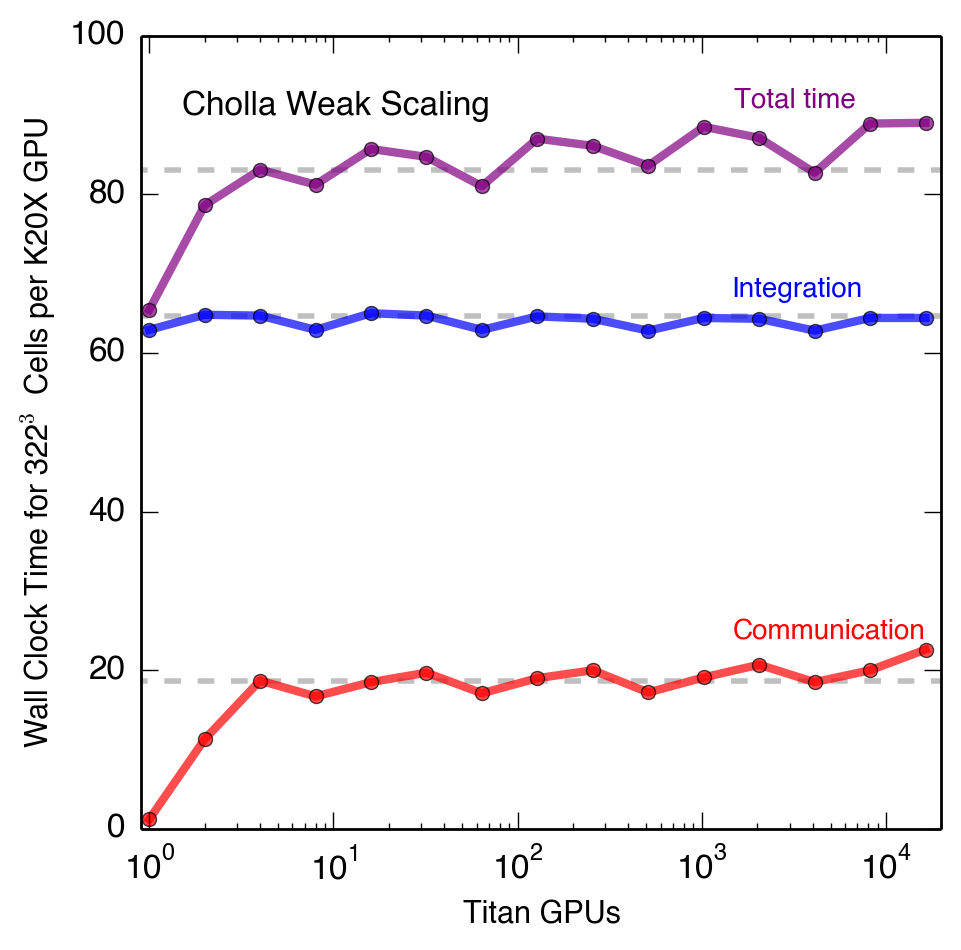
\includegraphics[width=4.52in, height=3.08in, keepaspectratio=true]{weak_scaling_adiabatic.png}
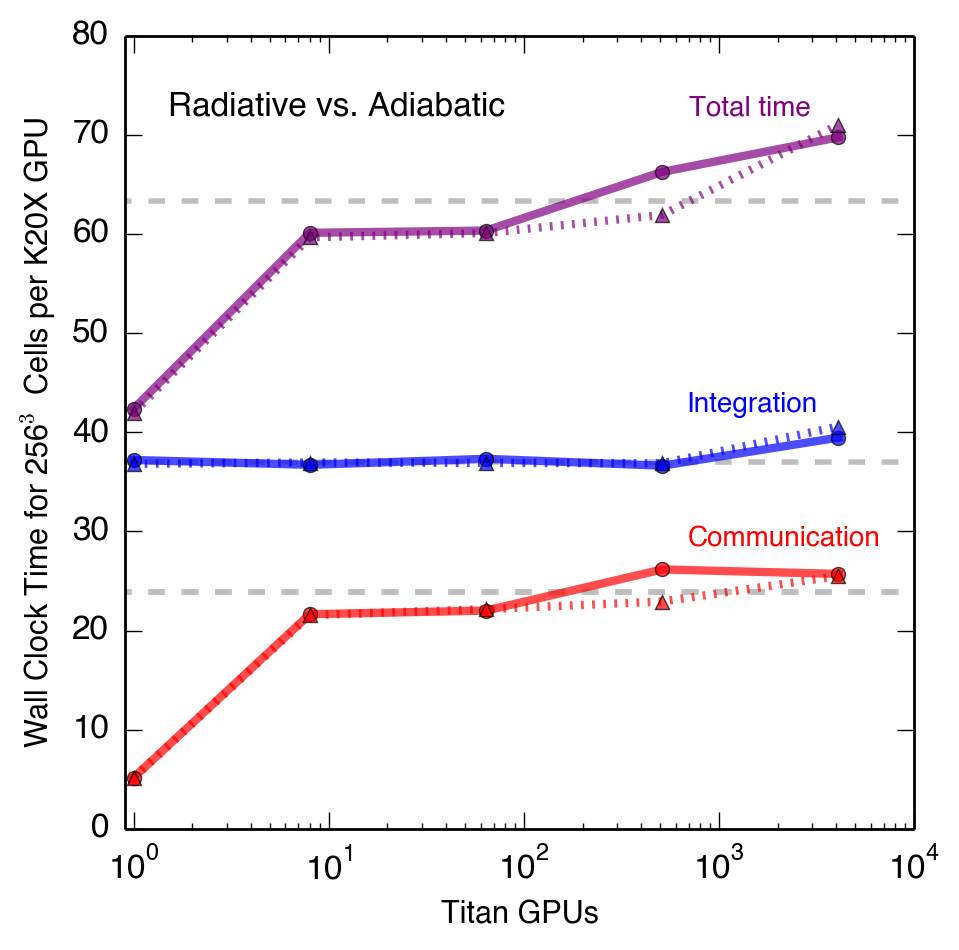
\includegraphics[width=4.52in, height=3.08in, keepaspectratio=true]{weak_scaling_radiative.png}
\caption{Weak scaling tests with {\tt Cholla} on Titan. Shown is the wall clock
execution time for an acoustic wave propagation test simulation when the
number of cells per GPU is kept fixed ($322^3$, left panel; $256^3$, right panel).
The code exhibits excellent weak scaling over four orders of magnitude in GPU (node) number, up to
16,384 Titan nodes tested. The largest simulation run in this test contained
$>0.5$T cells. The total simulation (purple), hydro algorithm (blue), and communications plus boundary conditions (red) timings are shown separately for comparison. In each case, the ideal scaling would be constant (gray dashed lines). Our novel GPU hardware-accelerated 
implementation of radiative cooling (right panel) allows for radiative simulations (dotted lines, triangles) to match otherwise identical 
adiabatic simulations (solid lines; circles) in computational
efficiency and weak scaling, as tested to 4096 GPUs.}
\label{fig:weak_scaling}
\end{figure}

We have implemented a novel GPU-accelerated radiative cooling scheme into {\tt Cholla} that uses the texture memory on the GPU
to perform linear interpolation on pre-computed cooling tables as a function of the gas density and temperature. The right
panel of Figure~\ref{fig:weak_scaling} compares the timing of adiabatic (solid) and radiatively-cooling (dotted) sound wave
propagation tests using $256^3$ cells per GPU on the Titan XK7 system, and demonstrates that the weak scaling performance
of the {\tt Cholla} code is nearly identical with or without radiative cooling. These tests are very similar to the calculations that will be performed 
in our turbulent CGM simulations, giving us additional confidence in our estimated run time for the petascale simulations that require optically-thin radiative cooling.


\vspace{-.25in}
\subsection{Developmental Work}
\vspace{-.2in}

%For the computational approach above, describe what, if any, development work has been carried out to date, especially on the architecture of the requested resource. Describe what development work will be executed, and when, during the proposed INCITE campaign, and an estimate of the computational resources required for this work.  If applicable, identify the milestones and production simulations in Section 2.3.i that are dependent on the developmental work and provide a plan for validating this developmental work.
Most of the developmental work for this program has either already been completed, or will be complete by the start of 2019. However, we highlight below some of the additional physics modules in {\tt Cholla} that will be used in this work, particularly those that we may improve over the coming months.

\vspace{-.2in}
\subsubsection{Cooling: COMPLETED}
\vspace{-.25in}


Since the publication of \cite{Schneider15}, a primary developmental task for the {\tt Cholla} codebase was
 the now-completed implementation of a model for optically-thin cooling. This task formed much of the motivation for
our DD Project AST119 granted in January 2016. This developmental work is complete and is
described in \cite{Schneider17}. Algorithmically, energy losses due to radiative cooling are precomputed using the
{\tt Cloudy} code \cite{Ferland13} assuming solar metallicity and a photoionizing
cosmic UV background. The cooling rates are stored in a two-dimensional table,
and interpolated as a function of gas density and temperature. This interpolation 
is GPU-accelerated by storing the table in texture memory on the GPU, which allows
for interpolation to be performed natively by the hardware using the CUDA {\tt cudaTextureObject\_t} and {\tt tex2D} capabilities.
We also use timestep subcycling combined with a forward-Euler integration to account for short cooling timescales in high density gas and radiative shocks. Even when several subcycles are required, this method of calculating radiative cooling remarkably adds negligible computational cost, allowing the superior
weak scaling of {\tt Cholla} to be maintained (see Figure \ref{fig:weak_scaling}).

\vspace{-.2in}
\subsubsection{Turbulence Generator: In Progress}
\vspace{-.25in}

As demonstrated in Figure\ref{fig:turbulence}, a turbulence generator has already been built for {\tt Cholla}. The current model imposes a series of ``kicks" to the velocities of each cell, with the energy injection rate normalized to offset energy losses due to radiative cooling. The velocity perturbations are applied over the course of a single time step at discreet intervals, typically 1/10th of the turbulent crossing time, $\Delta t = 0.1 L / c_s$. In addition to the kick model, this work will make use of a "constant energy injection" mode of turbulence driving that is currently under construction. In the constant energy model, kinetic energy is re-added to the grid at the end of each time step in an amount that exactly balances the global radiative losses. Co-PI Fielding has experience implementing this sort of turbulence generator, and will implementing it in {\tt Cholla}.

\vspace{-.2in}
\subsubsection{Conduction: In Progress, Supplemental}
\vspace{-.25in}

While not strictly required for the simulations outlined in this proposal, conduction is an additional physical process that may have a large effect on the physical state of gas in the circumgalactic medium. As such, we have begun development work on a conduction module for {\tt Cholla}, which will allow us to further explore the nature of thermal instability. This development is being done in conjunction with our current INCITE project (AST125), and as such, will be complete by the end of 2018. We expect to use conduction in a subset of the parameter study simulations for comparison purposes.

\vspace{-.3in}
\section{REFERENCES}
\vspace{-.3in}

%References are optional and may be structured in accordance with any style. They {\bf \em {do not}} count toward the 15-page limit.
\vspace{-.15in}

{\footnotesize
\bibliographystyle{usrt}
\renewcommand{\section}[2]{}
\begin{thebibliography}{500}
\bibitem{McCourt18} McCourt, M., et al. ``A characteristic scale for cold gas." {\em MNRAS}, {\bf 473}, 5407 (2018).
\bibitem{Fielding17} Fielding, D., et al. ``The Impact of Star Formation Feedback on the Circumgalactic Medium." {\em MNRAS}, {\bf 466}, 3810 (2017).
\bibitem{Godunov59} Godunov, S., ``A Difference Scheme for Numerical Solution of Discontinuous Solution of Hydrodynamic Equations.'' {\em Math. Sbornik}, {\bf 47}, 271 (1959)
\bibitem{Putman12} Putman, M.~E., Peek, J.~E.~G., \& Joung, M.~R.\ 2012,  ``Gaseous Galaxy Halos", {\em ARAA}, 50, 491 
\vspace{-.09in}
\bibitem{Schneider15} Schneider, E. and Robertson, B., ``{\tt Cholla}: A New Massively Parallel Hydrodynamics Code for Astrophysical Simulation'', {\em ApJS}, {\bf 217}, 24 (2015).
\vspace{-.09in}
\bibitem{Ferland13} Ferland, G., et al. ``The 2013 Release of Cloudy.'' {\em RMAA}, {\bf 49}, 137 (2013)
\vspace{-.09in}
\bibitem{Schneider17} Schneider, E. and Robertson, B., ``Hydrodynamical Coupling of Mass and Momentum in Multiphase Galactic Winds'', {\em ApJ}, {\bf 834}, 144 (2017).
\vspace{-.09in}
\bibitem{Steidel10} Steidel, C., et al. ``The Structure and Kinematics of the Circumgalactic Medium from Far-ultraviolet Spectra of z~=2-3 Galaxies.'' {\em ApJ}, {\bf 717}, 289 (2010)
\bibitem{Tumlinson17} Tumlinson, J., Peeples, M.~S., \& Werk, J.~K.\ 2017,  ``The Circumgalactic Medium", {\em ARAA}, 55, 389 
\vspace{-.09in}
\end{thebibliography}
}



\end{document}
